%-----------------------------------------------------------------
% LaTeX template for a document
% Written By: Pierre-Louis GAUTIER
% Date Updated: August 21, 2021 (v1.2.1)
%-----------------------------------------------------------------

\documentclass[a4paper, 11pt]{article}

% NOTE To conserve the space in the sentence passed as option to the package double braces to protect the spaces.
% It's an unfortunate feature of the core latex option handling

\usepackage[imageHeaderLeft     =   {clearWayShort.png},
            imageHeaderRight    =   {eseoShort.jpg},
            subject             =   {{}},
            keywords            =   {{}},
            encoding            =   {utf8},
            language            =   {french},
            showunnemberred     =   false
            ]{Parameter}

\usepackage[logoSchool  =   {eseoLong.jpg},
            logoCompany =   {clearWayLong.png},
            nameCompany =   {{ClearWay}},
            nameSchool  =   {{École d'Électronique de l'Ouest}},
            version     =   {0.0.1},
            status      =   {{En cours}},
            texte       =   {{}}
            ]{FrontPage}

%%%%%%%%%%%%%%%%%%%%%%%%%%%%%%%%%%%%%%%%%%%%%%%%%%%%%%
%% Load the glossary from the given files %%

\newignoredglossary{ignored}

\makeglossaries
\loadglsentries{glossary.tex}
\loadglsentries[ignored]{glossary-ignored.tex}

%% Load the bibliography from the given files %%

\addbibresource{biblio.bib}

%% General config for header, footer and front page %%

\author{\glsentryname{leo}, \glsentryname{damien}, \glsentryname{pierreLouis}}
\title{Guide d'installation de \glsentryname{sae}}
\date{\normalsize\today} % Enter a custom date or let it, it's the current date

%%%%%%%%%%%%%%%%%%%%%%%%%%%%%%%%%%%%%%%%%%%%%%%%%%%%%%

\begin{document}

\maketitle

\newpage
\pagenumbering{arabic} % restart the page numbering
\thispagestyle{empty}

\begin{table}[ht]
    \centering
    \begin{xltabular}{\linewidth}{| c
        | >{\centering\arraybackslash}X
        | >{\centering\arraybackslash}p{2.1cm}
        | c|}

        \hline
        \rowcolor{tableColorDark}  Date & Action                                 & Auteur               & Version
        \endfirsthead
        \hline

        06 janvier 2022                 & Création du document                  & \gls{pierreLouis}    & v0.0.1  \\\hline
        06 janvier 2022                 & Rédaction du guide d'installation     & \gls{pierreLouis}    & v0.1.0  \\\hline
        07 janvier 2022                 & Rédaction du guide d'utilisation      & \gls{damien}         & v0.1.1  \\\hline
        07 janvier 2022                 & Ajout des arguments, options et toml  & \gls{damien}         & v0.1.2  \\\hline


    \end{xltabular}
    \label{tab:versionning}
\end{table}


\newpage
\tableofcontents

\newpage
\part{Guide d'installation}

L'installation de \gls{sae} nécessite l'installation de \gls{python} et de \gls{pip}.\\
La version minimale de \gls{python} demandé est \textbf{3.7.*}, les versions \textbf{3.9} et supérieur n'ont pas été
testées.\\
Référer vous à la documentation de votre distribution (ou OS) pour savoir comment les installer.

\section{Depuis les fichiers sources}

Dans toute cette section, nous considérons que le terminal est placé au niveau du dossier du projet.

\begin{minted}{bash}
    cd path/vers/le/dossier/du/projet
\end{minted}

\subsection{Installation des \glsentryplural{paquet}}

Afin de pouvoir utiliser \gls{sae}, certains \glspl{paquet} sont nécessaires.\newline

L'installation des \glspl{paquet} peut être rapidement faite en utilisant le fichier \verb=requirements.txt= se
trouvant à la racine du projet :

\begin{minted}{bash}
    python3 -m pip install -r requirements.txt
\end{minted}

\subsubsection{Liste des \glsentryplural{paquet}}

\begin{itemize}
    \item Formater et linter
          \begin{description}
              \item[black] Formateur de code \gls{python} \cite{black}
              \item[flake8] Combinaison d'outils pour vérifier la code par rapport au style de codage PEP8
                  \cite{flake8, pep8}
                  \begin{description}
                      \item[flake8-bandit] Tests de sécurité automatisés \cite{flake8_bandit}
                      \item[flake8-import-order] Vérifie l'ordre de vos importations \cite{flake8_import_order}
                      \item[flake8-docstrings] Vérifie la conformité aux conventions des \gls{docstring} \gls{python}
                          \cite{flake8_docstrings}
                      \item[flake8-bugbear] Trouve les probables bogues et problèmes de conception dans le code
                          \cite{flake8_bugbear}
                      \item[flake8-return] Vérifie les valeurs de retour des fonctions dans le code \cite{flake8_return}
                      \item[pep8-naming] Vérifie le code par rapport aux conventions de nommage PEP8 \cite{pep8_naming, pep8}.
                  \end{description}
              \item[mypy]
                  Vérificateur de type statique pour \gls{python}. \cite{mypy}.
          \end{description}

    \item Nécessaire pour le fonctionnement
          \begin{description}
              \item[transitions] Une implémentation légère et orientée objet de la machine à états en \gls{python} \cite{transition}
              \item[RPi.GPIO] Fournit une classe pour contrôler le GPIO sur une Raspberry Pi \cite{rpi_gpio}.
                  {\color{red}Il ne sera pas installé avec le fichier \verb=requirements.txt=, car non disponible pour
                  les architectures autres que ARM}
              \item[imutils] Une série de fonctions de commodité pour rendre les fonctions de traitement d'image de
                  base \cite{imutils}
              \item[numpy] Permet d’effectuer des calculs numériques avec \gls{python} \cite{numpy}
              \item[opencv-python] Bibliothèque open-source pour la vision par ordinateur, l'apprentissage automatique
                  et le traitement des images \cite{opencv}
              \item[toml] Analyse et créer des fichierl TOML \cite{toml}
              \item[Mock.GPIO] Bibliothèque de \glspl{mock} pour la bibliothèque \gls{python} \textit{RPI.GPIO} \cite{mock_gpio}.
          \end{description}

    \item Nécessaire pour les tests
          \begin{description}
              \item[pytest] \Gls{framework} permettant d'écrire facilement des tests petits et lisibles \cite{pytest}
              \item[pytest-cov] Produit un rapport de couverture avec de tests réalisés avec \textit{pytest} \cite{pytest_cov}
              \item[pytest-mock] Fournit un injecteur de \gls{mock} \cite{pytest_mock}
              \item[flake8-pytest-style]
                  Vérifie les problèmes de style communs ou les incohérences \cite{flake8_pytest_style}.
          \end{description}

    \item Nécessaire pour la génération du \gls{paquet} du \gls{sae}
          \begin{description}
              \item[build] Outil de construction simple qui n'effectue aucune gestion des dépendances. \cite{build}
          \end{description}
\end{itemize}


\section{Installation avec \glsentryname{pip}}


\newpage
\section{Branchements des composants au Raspberry}
Le \gls{RPiCard} doit être alimenté avec une alimentation secteur. Un switch permet d'éteindre et d'allumer la carte.

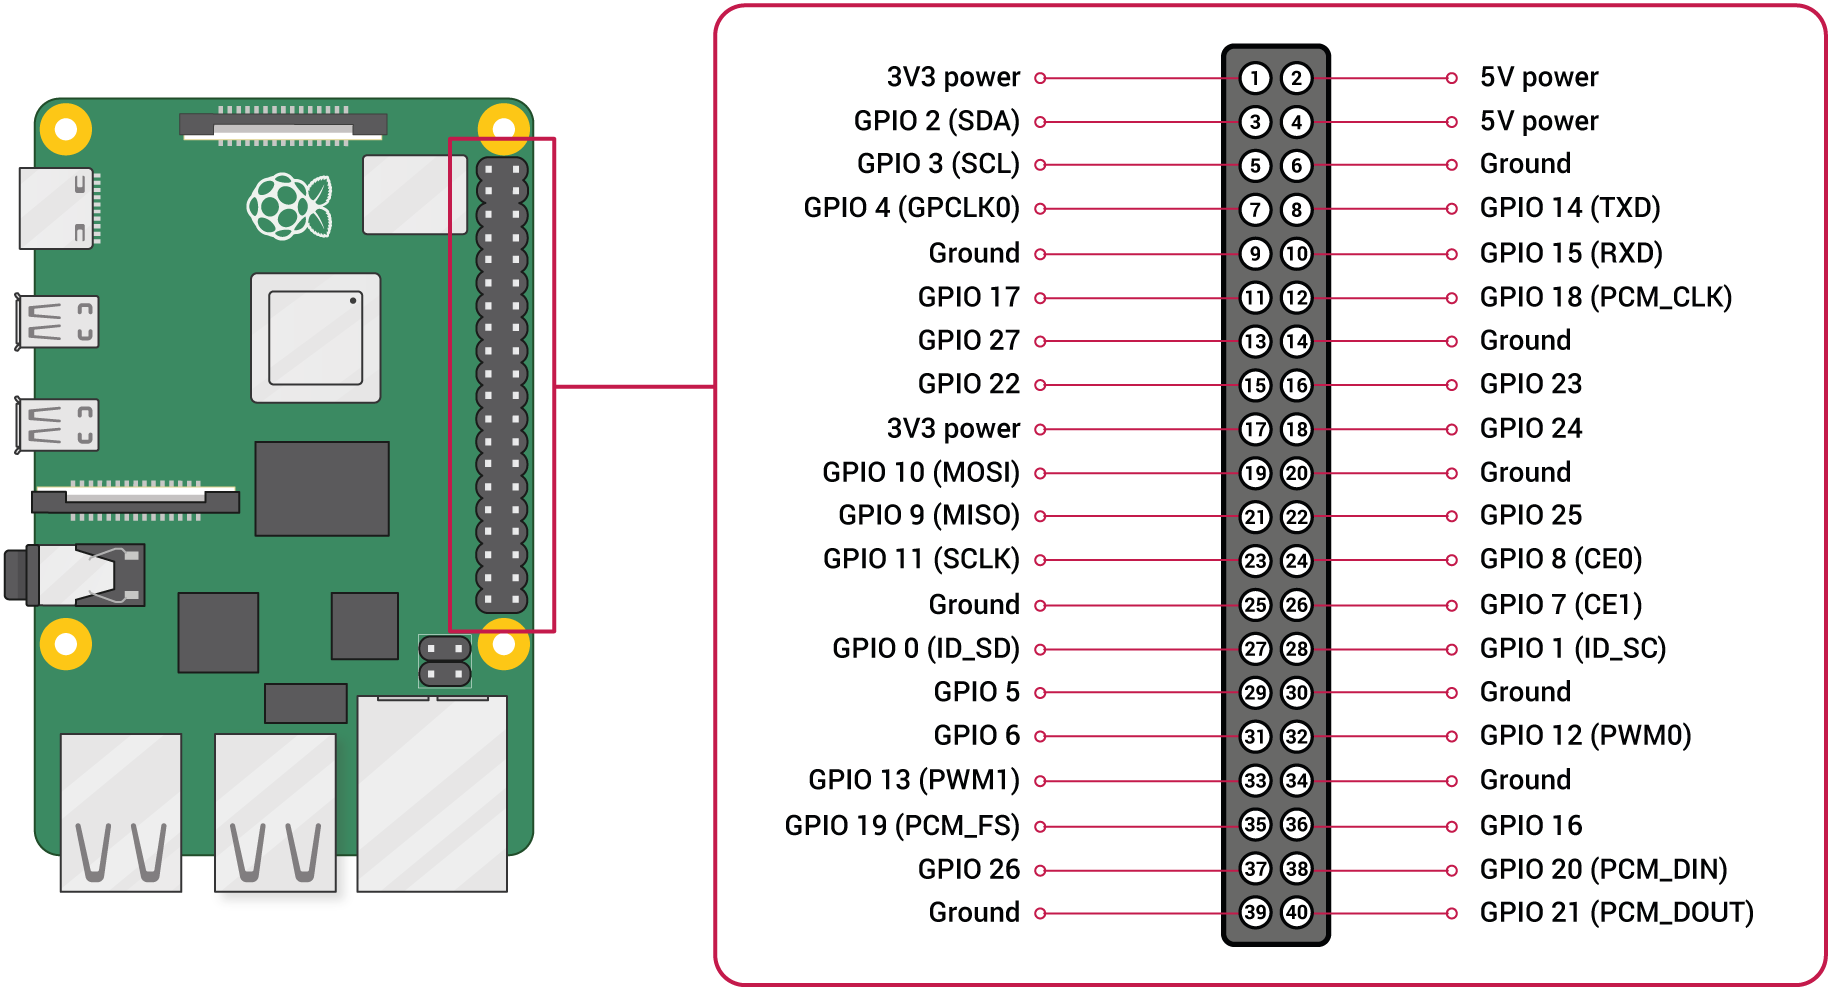
\includegraphics[width=\textwidth]{img/Rpi4_pin.png}

\subsection{Branchements du servomoteur}

Pour le logiciel fournit, le servomoteur \gls{SG90} a des branchements spécifiques.
\begin{itemize}
    \item Fil marron : GND
    \item Fil rouge  : 5V
    \item Fil orange : GPIO 12
\end{itemize}

\subsection{Branchements du panneau de LEDs}

En considérant que vous êtes dos au panneau :
\begin{itemize}
    \item Brancher la borne de droite du bornier à la broche GPIO 5
    \item La borne du milieu doit rester vide
    \item Brancher la borne de gauche du bornier au GND
\end{itemize}

\subsection{Branchements de la caméra}
La caméra \gls{RPiCamera} est fournie avec une nappe. Côté caméra : Ouvrer le connecteur d'accueil de nappe en tirant sur la languette. 
Positionner la nappe de façon à ce que le trait de couleur bleu soit au dos de la lentille et fermer le connecteur. 
Faire de même sur le port d'accueil caméra du \gls{RPiCard}. Positionner le trait bleu face au connecteur Ethernet.


\newpage
\part{Guide d'utilisation}
La présente section a pour but de décrire l'utilisation du \gls{sae}.

\section{\glsentryname{sae} - Description du service}
\label{sec:description_clearWay}

\gls{sae} est composé de trois éléments :
\begin{itemize}
    \item Le module caméra comprend une caméra (\gls{RPiCamera}), un socle en bois, un servomoteur (\gls{SG90})
          et un dispositif en plastique permettant de faire la liaison entre le servomoteur et la caméra.
    \item Un boîtier noir où se trouve une carte \gls{RPiCard}.
    \item Le panneau en bois intégrant des LEDs permettant les automobilistes qu'un cycliste arrive.
\end{itemize}

\section{Exécution de \glsentryname{sae}}
\label{sec:execution_clearWay}

\gls{sae} est actuellement un prototype.

\subsection{Utilisation du \glsentrytext{ssh}}
\label{sec:utilisationSSH}

Pour une exécution sur la \gls{raspberry} à distance, il faut établir une connexion \gls{ssh}
Pour se faire, le plus simple est d'être connecté au même réseau que cette dernière.

\subsubsection{Trouver l'adresse \glsentrytext{ip}}
\label{sec:trouverIP}

\paragraph{À partie du \textit{hostname}}

Si vous connaissez le \textit{hostname} de votre \gls{raspberry} : \mintinline{bash}{ping <hostname>.local}.\\
L'adresse \gls{ip} s'affichera dans le terminal.

\subparagraph{Exemple}

Pour une \gls{raspberry} dont le \textit{hostname} est \underline{raspberrypi} (valeur par défaut à
l'installation) :

\begin{minted}{bash}
            $ ping raspberrypi.local

            PING raspberrypi.local (123.123.123.123) 56(84) octets de données.
            64 octets de par10s33-in-f14.1e100.net (123.123.123.123) : icmp_seq=1 ttl=115 temps=19.3 ms
            64 octets de fra02s18-in-f14.1e100.net (123.123.123.123) : icmp_seq=2 ttl=115 temps=24.3 ms
            ...
\end{minted}

L'\gls{ip} nous est alors donné et est \texttt{123.123.123.123}.

\paragraph{À partie de votre adresse \glsentrytext{ip}}

Sinon retrouver votre adresse \gls{ip}\footnote{Référer vous à la documentation de votre OS}, afin de déterminer
la plage de sous-réseau, le et utiliser la commande \mintinline{bash}{nmap -sn <subnet>/24}.
L'ensemble des appareils sur votre réseau seront "pinger" :

\subparagraph{Exemple}

Si mon \gls{ip} est \texttt{123.123.123.5} alors mon sous-réseau est \texttt{123.123.123.0}.

\begin{minted}{text}
            # sudo nmap -sn 123.123.123.0/24

            Starting Nmap 7.92 ( https://nmap.org ) at 2022-01-07 14:58 EAT
            Nmap scan report for 123.123.123.1
            Host is up (0.0055s latency).
            MAC Address: 50:0F:F5:3E:22:50 (Unknown)
            Nmap scan report for 123.123.123.106
            Host is up (0.010s latency).
            MAC Address: C4:D9:87:BA:88:17 (Intel Corporate)
            Nmap scan report for 123.123.123.105
            Host is up.
            MAC Address: B8:37:EB:EA: E0:D5 (Raspberry Pi Foundation)
            Nmap scan report for 123.123.123.200
            Host is up (0.0049s latency).
            Nmap done: 256 IP addresses (4 hosts up) scanned in 205.26 seconds.
\end{minted}

Dans notre exemple ci-dessus, la commande \texttt{nmap} a trouvé un périphérique \gls{raspberry} :

\begin{minted}{text}
    MAC Address: B8:37:EB:EA: E0:D5 (Raspberry Pi Foundation)
    Nmap scan report for 123.123.123.200
\end{minted}

\subsubsection{Connexion}

Pour se connecter en \gls{ssh} à la \gls{raspberry}, il faut connaitre l'utilisateur\footnote{Par défaut sur une
    \gls{raspberry}, l'utilisateur est \underline{pi}.} auquel on veut se connecter et l'\gls{ip} de la \gls{raspberry}
(voir section \nameref{sec:trouverIP}).\\
La commande à exécuter est :

\begin{minted}{bash}
    ssh <user>@<ip_address>
\end{minted}

Il vous sera alors demandé de confirmer si vous souhaiter vous connecter, et ensuite, le mot de passe de
l'utilisateur\footnote{Par défaut pour l'utilisateur \underline{pi}, le mot de passe est \underline{raspberry}}.

\paragraph{Copie de fichier de l'ordinateur vers la \glsentryname{raspberry}}
\label{sec:copieVersRaspberry}

Pour copier un fichier depuis votre ordinateur vers la \gls{raspberry} (ou une quelconque cible distante), il faut
utiliser la commande \texttt{scp} qui utilise le \gls{ssh}.\\
La commande est :

\begin{minted}{bash}
    scp <file_to_send> <user>@<ip_address>:<path_on_the_raspberry>
\end{minted}

\subsection{Arguments nécessaires pour l'exécution du programme}
\label{sec:executionArg_clearWay}
Certains arguments sont nécessaires afin d'utiliser \gls{sae}. La liste ci-dessous répertorie ces derniers.

\begin{table}[H]
    \centering
    \rowcolors{2}{tableColor}{white}
    \begin{tabularx}{\linewidth}{|c|X|c|}
        % Header
        \hline
        \rowcolor{tableColorDark} Argument      & Signification                                                                                                                                             & Support              \\
        \hline
        % Data
        \texttt{-{}-yolo-weights YOLO\_WEIGHTS} & Requis si l'argument \texttt{-{}-config} n'est pas renseigné. Chemin vers le fichier yolo-weights                                                         & Raspberry Ordinateur \\\hline
        \texttt{-{}-yolo-cfg YOLO\_CFG}         & Requis si l'argument \texttt{-{}-config} n'est pas renseigné. Chemin vers le fichier yolo-cfg                                                             & Raspberry Ordinateur \\\hline
        \texttt{-{}-size SIZE}                  & Requis si l'argument \texttt{-{}-config} n'est pas renseigné. La taille de l'image (320 ou 416 recommandés).                                              & Raspberry Ordinateur \\\hline
        \texttt{-{}-config CONFIG}              & (Utilisable avec l'alias \texttt{-c CONFIG}) Chemin vers le fichier de configuration. À utiliser si les trois arguments précédents n'ont pas été précisés & Raspberry Ordinateur \\\hline
    \end{tabularx}
    \label{tab:ArgClearway}
    \caption{Argument d'exécution de \gls{sae}}
\end{table}

\subsection{Options possibles pour le programme}
\label{sec:executionOption_clearWay}
\gls{sae} est livré avec plusieurs options à renseigner lors du démarrage du programme. La liste ci-dessous répertorie ces dernières.

\begin{table}[H]
    \centering
    \rowcolors{2}{tableColor}{white}
    \begin{tabularx}{\linewidth}{|c|X|c|}
        % Header
        \hline
        \rowcolor{tableColorDark} Option              & Signification                                                                                                                                              & Support              \\
        \hline
        % Data
        \texttt{-{}-camera\_angle}                    & Renseigner l'angle de la caméra en degrés.                                                                                                                 & Raspberry            \\\hline
        \texttt{-{}-help}                             & (Utilisable avec l'alias \texttt{-h}) Affiche les arguments et options possibles.                                                                          & Raspberry Ordinateur \\\hline
        \texttt{-{}-input-path INPUT\_PATH}           & (Utilisable avec l'alias \texttt{-i INPUT\_PATH}) Chemin vers la vidéo à analyser si la caméra n'est pas utilisée                                          & Raspberry Ordinateur \\\hline
        \texttt{-{}-no-gpio}                          & Les GPIOs ne seront pas utilisés. Uniquement les logs seront affichés.                                                                                     & Raspberry Ordinateur \\\hline
        \texttt{-{}-on-raspberry}                     & Informe le programme que le Raspberry sera utilisée                                                                                                        & Raspberry            \\\hline
        \texttt{-{}-output-path OUTPUT\_PATH}         & (Utilisable avec l'alias \texttt{-o OUTPUT\_PATH}) Chemin vers le dossier qui contraindra la vidéo analysée (inclut les boxes autours des objets détectés) & Raspberry Ordinateur \\\hline
        \texttt{-{}-panel-gpios PANEL\_GPIOS}         & Informe le programme quel(s) GPIO(s) utiliser, sous forme d'une liste                                                                                      & Raspberry            \\\hline
        \texttt{-{}-see-rtp}                          & Permet d'avoir une fenêtre avec l'analyse en temps réelle.                                                                                                 & Raspberry Ordinateur \\\hline
        \texttt{-{}-servo-gpio}                       & Permet d'indiquer la broche GPIO utilisé par le servomoteur.                                                                                               & Raspberry            \\\hline
        \texttt{-{}-use-gpio}                         & Les GPIOs seront utilisés, les logs seront également affichés.                                                                                             & Raspberry            \\\hline
        \texttt{-{}-verbosity \{WARNING,INFO,DEBUG\}} & (Utilisable avec l'alias \texttt{-v \{WARNING,INFO,DEBUG\}}) Indique le niveau de verbosité.                                                               & Raspberry Ordinateur \\\hline
        \texttt{-{}-version}                          & (Utilisable avec l'alias \texttt{-V}) Affiche la version de \gls{sae}                                                                                      & Raspberry Ordinateur \\\hline
    \end{tabularx}
    \label{tabOptClearway}
    \caption{Options d'exécution de \gls{sae}}
\end{table}

Exemple de la ligne de commande pour utiliser les paramètres par défauts :

\begin{minted}{bash}
    clearway --yolo-weights resources/yolov2-tiny.weights --yolo-cfg  resources/yolov2-tiny.cfg
\end{minted}

\subsection{Champs du fichier \textbf{TOML}}
\label{sec:executionTOML_clearWay}

\gls{sae} est livré avec un fichier \textbf{TOML} permettant de configurer le système.

\begin{table}[H]
    \centering
    \rowcolors{2}{tableColor}{white}
    \begin{tabularx}{\linewidth}{|c|X|c|}
        % Header
        \hline
        \rowcolor{tableColorDark} Fichier \textbf{TOML}  & Signification                                                                                                                & Support              \\
        \hline
        % Data
        \texttt{camera\_angle = 90}                  & Renseigner l'angle de la caméra en degrés                                                                                                                         & Raspberry               \\\hline
        \texttt{format = "Format\_Type"}             & Format du fichier de logging, \href{https://docs.python.org/3/howto/logging-cookbook.html\#formatting-styles}{documentation}                                      & Raspberry Ordinateur    \\\hline
        \texttt{on-raspberry = false}                & Informe le programme que le Raspberry sera utilisée                                                                                                               & Raspberry               \\\hline
        \texttt{path = "clearway.log"}               & Chemin où sera sauvegardé le fichier des logging                                                                                                                  & Raspberry               \\\hline
        \texttt{panel = [5, 7]}                      & Informe le programme quel(s) GPIO(s) utiliser, sous forme d'une liste                                                                                             & Raspberry               \\\hline
        \texttt{see-rtp = false}                     & Permet d'avoir une fenêtre avec l'analyse en temps réelle                                                                                                         & Raspberry Ordinateur    \\\hline
        \texttt{servo\_gpio = 17}                    & Permet d'indiquer la broche GPIO utilisé par le servomoteur                                                                                                       & Raspberry               \\\hline
        \texttt{size = 416}                          & La taille de l'image (320 ou 416 recommandés).                                                                                                                    & Raspberry Ordinateur    \\\hline
        \texttt{use-gpio = false}                    & Les GPIOs seront utilisés, les logs seront également affichés.                                                                                                    & Raspberry               \\\hline
        \texttt{verbosity = "DEBUG"}                 & Indique le niveau de verbosité                                                                                                                                    & Raspberry Ordinateur    \\\hline
        \texttt{yolo\_cfg = "yolov2.cfg"}            & Chemin jusqu'au fichier .cfg de yolo                                                                                                                              & Raspberry Ordinateur    \\\hline
        \texttt{yolo\_weight = "yolov2.weight"}      & Chemin jusqu'au fichier .weight de yolo                                                                                                                           & Raspberry Ordinateur    \\\hline
    \end{tabularx}
    \label{tab:tomlClearway}
    \caption{Argument d'exécution de \gls{sae}}
\end{table}

Exemple complet du contenu possible d'un fichier \textbf{TOML} fonctionnel :

\begin{minted}{toml}
    [clearway]
    [clearway.gpio]
    use_gpio = false
    panel_gpios = [5, 6]
    camera_angle = 75
    servo_gpio = 12
    [clearway.ai]
    yolo_cfg = "resources/yolov2-tiny.cfg"
    yolo_weights = "resources/yolov2-tiny.weights"
    on_raspberry = false
    size = 320
    see_rtp = false
    [clearway.log]
    verbosity = "DEBUG"
    format = "%(asctime)s [%(filename)s:%(lineno)d] %(levelname)s >> %(message)s"
    path = "clearway.log"
\end{minted}

\newpage
\part*{Annexes}
\listoffigures
\listoftables

\newpage
\printglossary % Display the glossary, see the documentation for the options

\newpage
\printbibliography % Display the bibliography, see the documentation for the options

\end{document}
